% CONCLUSIONS
\chapter*{Synthèse et perspectives}
\markboth{Synthèse et perspectives}{}
\addcontentsline{toc}{chapter}{Conclusions et perspectives}
\newpage

%L'étude des flux de carbone dans les écosystèmes tourbeux est complexe car assujetti à des facteurs de contrôle dont la prépondérance varie fortement selon l'échelle considérée et les conditions environnementales.
%Les effets d'un facteur contrôlant sur un flux de gaz vont généralement dans le même sens dans la littérature : 
%une hausse de la température à tendance à augmenter les flux.
%Une augmentation du niveau de la nappe à tendance à favoriser la production de \chh par rapport à celle du \coo.
%La végétation semble faciliter les échanges de gaz et libère des substrats facilement mobilisables.
%Outre le fait que ces facteurs co-varient et qu'il donc difficile de distinguer leurs effets, ces effets sur les différents flux en terme de bilan de carbone est beaucoup moins nette, d'où la nécessité d'estimer des bilans de carbone sur ces écosystèmes.


Le devenir des tourbières, de leur fonction de puits et de leur stock de carbone accumulé pendant les derniers millénaires, reste incertain.
Ces travaux se sont focalisés sur l'étude d'une tourbière de Sologne (la tourbière de La Guette), envahie par une végétation vasculaire.
L'intérêt de son étude réside dans cette problématique de perturbation anthropique probablement liée à cet envahissement.
Mais également sa position à la limite sud de l'extension des tourbières à sphaignes de l'hémisphère Nord, qui la place dans des conditions limites, moins favorable a priori au développement de ces écosystèmes.

\section*{Synthèse générale}

\subsection*{Intensité des flux sur la tourbière de La Guette}

%\subsubsection{Intensité des flux sur la tourbière de La Guette}
Les estimations des flux de \coo sur la tourbière de La Guette sont dans la tranche haute des émissions relevées dans la littérature que ce soit pour la RE ou la PPB.
Il semble cohérent que les flux de \coo soient plus fort que ceux mesurés dans des tourbières boréales.
De par sa position géographique, le site à une température moyenne annuelle élevée par rapport à la majorité des écosystèmes tourbeux.
La tourbière subit également un climat moins dur avec des hivers moins longs et froids que celles situées à plus hautes latitudes, ce qui permet aux flux de rester plus fort pendant une période de l'année plus longue.
Les estimations des flux de \coo se rapprochent de celles estimées dans les tourbières utilisées comme prairies permanentes, sans toutefois les atteindre.
Ceci semble également cohérent car ces écosystèmes ont généralement un niveau de nappe d'eau plus bas.
En outre cette comparaison a du sens car la tourbière de La Guette, est fortement envahie par une herbacée (\textit{Molinia caerulea}) largement dominante.

Les flux de \chh estimés sont également importants et et plutôt dans la tranche supérieure des valeurs relevées dans la littérature.
%Ces observations sont cohérentes avec le niveau de nappe d'eau haut relevé sur le site pendant les deux années de mesure qui a contribuer à minimiser l'oxydation du \chh pendant son transport vers l'atmosphère.

Enfin les flux de COD sont contraint principalement, sur les deux années de mesures, par la quantité d'eau qui quitte l'écosystème supérieure en 2014 par rapport à 2013.

\subsubsection{Effet de l'hydrologie sur les flux de GES}

Même si les faibles variations du niveau de la nappe d'eau mesurée sur la tourbière de La Guette pendant les deux années de mesure n'ont pas permises de les relier directement aux émissions de GES, l'hydrologie joue un rôle important.
%Ainsi le niveau de nappe élevé en 2013 et 2014 explique probablement

D'abord l'importance de flux de \chh, dont l'estimation est plutôt dans la tranche supérieure des valeurs relevées dans la littérature, est probablement liée au niveau de la nappe d'eau.
Ce dernier en étant proche de la surface du sol empêche l'oxydation du \chh.
Le fait d'avoir des flux plus faible en 2013, année ou le niveau de nappe a légèrement baissé en été, qu'en 2014 va dans le même sens.
Suite aux expérimentations sur mésocosmes, il semble d'ailleurs qu'à niveau de nappe d'eau élevé, la proportion aérobie/anaérobie de la colonne de sol ne soit plus le processus prépondérant de contrôle des émissions de \chh.

? au dessus de -10 limitation car limitation de la photosynthèse ? (semble pas particulièrement minimiser dans chap4)

Ensuite malgré un niveau moyen de la nappe d'eau plus élevé en 2014 qu'en 2013, l'estimation de la quantité d'eau sortant de la tourbière est également supérieure en 2014.
Cette inconsistance s'explique probablement par l'histoire de la tourbière pendant les années précédents les mesures.
En 2011 et 2012 la tourbière a subit un étiage important et s'est vidée d'une part importante de son eau, suffisante pour pouvoir s'y déplacer sans bottes (Sébastien Gogo, communication personnelle), ce qui n'est jamais arrivé en 2013 et 2014.
En 2013 une partie importante de l'eau arrivant dans la tourbière a donc servie à la renflouer, cette part l'est beaucoup moins en 2014 la tourbière étant déjà en grande partie « en eau ».
Ces variations dans la décharge en eau de la tourbières sont la source des différences d'estimation du COD entre 2013 et 2014.
%Cette histoire semble expliquer les estimations des flux de COD, supérieur en 2014.

Enfin, même si aucune tendance directe n'est visible avec les flux de \coo, le niveau de la nappe d'eau particulièrement élevé pendant les deux années de mesure a probablement eu un rôle.
Notamment il a pu limiter un peu les flux de RE en minimisant la proportion aérobie de la colonne de tourbe.
Malgré tout les flux observés sont important, cela peut s'expliquer car à la fois \textit{Molinia caerulea} et \textit{Eriophorum Augustifolium} (\textbf{Vaginatum oui mais augustifolium ?}) possèdent un aérenchyme, cette adaptation aux milieux inondés, qui leur permet de maintenir des échanges gazeux de leurs racines à l'atmosphère.
Son effet est davantage visible sur les expérimentations sur mésocosmes, ou un niveau de la nappe d'eau plus bas entraîne une augmentation des émissions de la RE.
%Les flux de \chh ne semblent quant à eux pas être contraint par le niveau de la nappe pendant les deux années de mesures.
%Leur relation avec la végétation laisse encore une fois penser un effet possible de l'aérenchyme.

%\subsubsection{Contrôle du COD}

\subsection*{Le bilan de carbone}

Les estimations du bilan de carbone de la tourbière de La Guette montrent que l'écosystème tend à se comporter comme une source de carbone et ce malgré un niveau de nappe élevé.
Plusieurs points peuvent être avancés pour expliquer cela.
Le premier concerne les températures moyennes annuelles du site qui sont élevées par rapport à d'autres tourbières.
Ces températures entraînent des flux forts, que ce soit pour la PPB ou la RE.
La tourbière de La Guette est également une tourbière de plaine qui ne profite pas des été plus frais et humides et des hivers plus froids d'un climat montagnard par exemple.
Ceci peut jouer sur le bilan en augmentant la RE, notamment la nuit alors que la PPB s'arrête.
On peut ainsi comparer le premier jour des mesures haute fréquence entre les sites de Frasne et de La Guette (cf chapitre~\ref{ch:ch5}, Figure~\ref{fig:er_tair_tpeat}).
Les flux mesurés à Frasne ont un maximum moins élevé le jour et un minimum plus bas la nuit, alors que les température de l'air maximum de la journée sont plus forte à Frasne.
(Limites de la comparaison : mesure à un temps différent)
Enfin la présence d'une végétation vasculaire herbacée, ubiquiste, adaptée aux milieux inondés permet de maintenir une activité photosynthétique et de respiration.

%Explications : les températures moyennes annuelles qui favorise l'augmentation de RE (et de PPB mais que le jour).
%La position de la tourbière de LG, en plaine : par rapport à frasne (climat davantage montagnard) RE baisse moins la nuit sur les 3 jours de mesures (chap5) (la comparaison est limitée mais...)
%Autre explication la végétation vasculaire : a dvlper
Ce bilan est contrôlé en grande partie par les émissions de \coo qui sont deux ordres de grandeur au dessus de celles du \chh et du COD.
Pour les modèles PPB-1 et RE-1 on a :

\begin{equation}
100C_{PPB} \rightarrow 98C_{RE} + 1C_{\chh} + 1C_{COD} + 0\Delta C
\end{equation}

Soit pour 100 atomes de carbone assimilés par la photosynthèse, 98 émis sous forme de \coo respiré, 1 sous forme de \chh et 1 sous forme de COD et un bilan à l'équilibre.
Pour PPB-2 et RE-3 on a :

\begin{equation}
100C_{PPB} \rightarrow 118C_{RE} + 2C_{\chh} + 1C_{COD} -21\Delta C
\end{equation}

Soit pour 100 atomes de carbone assimilés par la photosynthèse, 118 émis sous forme de \coo respiré, 2 sous forme de \chh et 1 sous forme de COD et une perte de 21 atomes de carbone.
%\subsubsection*{Bilan de carbone}

\subsection*{variabilité spatiale des flux}

Ces travaux ont également montrés la forte variabilité spatiale des flux de \coo.
Le nombre limité de points de mesure du \chh ne permettant pas d'affirmer quoi que ce soit de ce côté là.
(\textbf{dvlpé var spa + vég})
Paradoxalement les zones de la tourbières fonctionnant en puits de carbone sont celles ou les herbacées sont dominantes.

\subsection*{Les modèles}

\subsubsection{Intérêt de l'évaluation}
%Cette force des flux de \coo est probablement liée à sa situation géographique locale et globale : une tourbière de plaine située à basse latitude et à ses problématiques de drainage et d'envahissement par une végétation vasculaire.
%Ainsi la saisonnalité plus faible qu'en montagne permet aux flux de rester fort pendant une période de l'année plus importante.
%Ces flux importants entraînent des variations forte en terme de bilan selon les méthodologies employées, il est cependant probable que la tourbière de La Guette fonctionne actuellement comme une source de carbone.

%L'estimation du bilan à l'échelle saisonnière ne permet pas de reproduire les variations journalières, l'estimation du modèle pendant les 3 jours de mesures haute fréquence réalisés en 2013 est largement supérieure aux valeurs mesurées (Figure~\ref{fig:RE1_vs_JN})

Que ce soit pour la PPB ou la RE, la prise en compte de la végétation améliore la calibration des modèles.
Pour la PPB l'intégration de la végétation n'améliore pas l'évaluation du modèle.
Ceci indique que, si d'autres suivis du même type sont effectués sur le site, l'estimation des flux de PPB en intégrant la végétation est à étudier à nouveau et ne va pas de soi.
De plus l'intégration de la végétation dans l'estimation des flux de PPB à un effet important qui change le bilan final de l'écosystème.
À l'inverse pour la RE l'intégration de la végétation, qui améliore également l'évaluation, ne change de façon importante l'estimation du flux de carbone.
Son utilisation pour estimer les flux de RE d'autres suivis du même type sur la tourbière de La Guette semble pertinent.
Enfin l'estimation du \chh, dont l'évaluation montre une erreur importante, doit être limité à l'estimation d'un ordre de grandeur des flux émis lors de ce suivi en particulier.
Ces résultats montrent l'intérêt fort de l'évaluation des modèles utilisés pour pouvoir préciser leur limites d'utilisation mais également les limites dans les interprétations qu'ils permettent.

La prise en compte de la végétation reste une difficulté importante, l'observation répétée nécessitant des mesures non destructives, souvent imprécises ou très coûteuses en temps.


\subsection*{Modélisation saisonnière et mesures horaires}

Les estimations des flux de la tourbière de La Guette par les modèles du chapitre~\ref{ch:ch3} ont été calculées à l'heure.
Elles ont donc pu être comparées aux données acquises sur le même site lors d'autres expérimentations, notamment grâce à l'utilisation de méthodes de mesures identiques sur l'ensemble de ces travaux.
Ainsi si l'on compare la RE estimée à l'aide des modèles RE-1 et RE-3 (chapitre~\ref{ch:ch3}) aux données acquises à haute fréquence (chapitre~\ref{ch:ch5}) on observe un écart important entre les valeurs mesurées et celles estimées par les modèles (Figure~\ref{fig:RE1_vs_JN}).
Pour expliquer cet écart on peut considérer les deux points suivants : 

Premier point, on compare des modèles qui prennent en compte la variabilité spatiale du site (une partie au moins, à travers les vingts points qui on servi à les calibrer) à des mesures réalisées sur quatre embases dans une zone restreinte de la tourbière (20 x \SI{20}{\metre}).
Ces quatre points ayant une représentativité spatiale limitée et ont été choisi pour leur similarités.
Cet écart peut donc être en partie le reflet de la variabilité spatiale des flux dans la tourbière.
Cet argument est soutenu par les mesures de RE réalisées le 24 et le 25 juillet 2013, soit 5 jours avant les mesures haute fréquence et dont la gamme de valeur est comprise entre \num{4.8} et \SI{18.9}{\uml} et sont représentés par le fond gris sur la figure~\ref{fig:RE1_vs_JN}.
Les estimations des modèles RE-1 et RE-3 restent d'ailleurs majoritairement dans cette gamme de valeurs.
Par ailleurs, la placette p04 (Figure~\ref{fig:carteVS}) la plus proche des mesures haute fréquences, est dans la gamme basse des flux que ce soit pour la campagne du 24-25 juillet : troisième flux le plus faible mesuré (\SI{6.1}{\uml}) ou en moyenne sur l'ensemble de mesure ou elle vaut \SI{2.81(160)}{\uml} par rapport à la moyenne de l'ensemble des placettes valant \SI{3.77(289)}{\uml}.

Second point, le modèle est calibré à partir de moyennes des flux par campagne de mesure (Figure~\ref{fig:ER_evolution_avg}).
Ces moyennes sont comprises entre \num{0.69(027)} et \SI{9.43(348)}{\uml}, par conséquent les estimations des modèles, dont RE-1, en dehors de cette gamme sont du domaine de l'extrapolation et donc à considérer avec précaution.

\begin{figure}
\centering
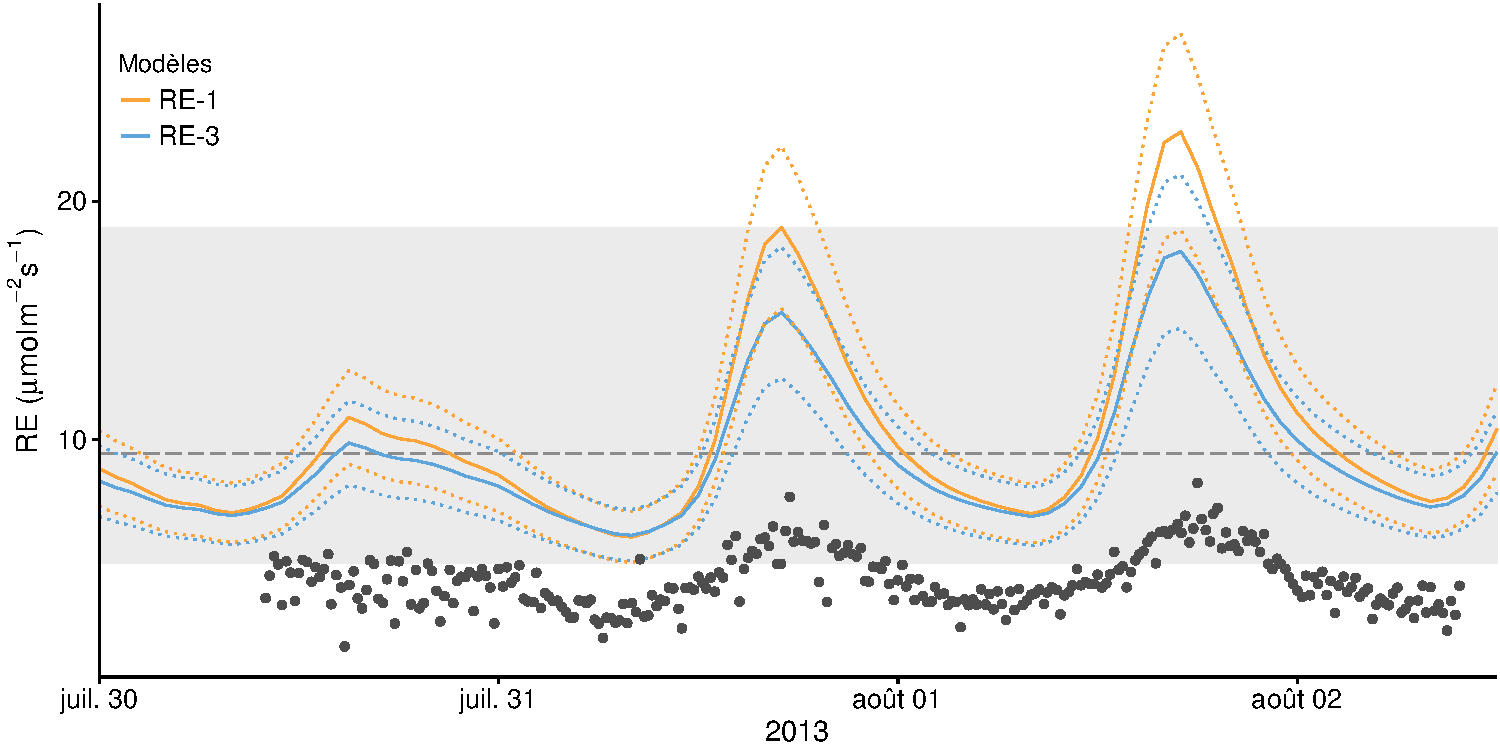
\includegraphics[width=1.15\textwidth, center]{conclusions/RE1_vs_JN}
\caption{Comparaison entre les valeurs estimées par les modèle RE-1 (ligne orange), RE-3 (ligne bleue) et les mesures faites à haute fréquence sur le site du 30 juillet au 2 août 2013 (points noirs). Les lignes de pointillés représentent l'erreur (NRMSE) associée aux modèles. La zone grisée correspond à la gamme de valeur de la RE mesurée sur l'ensemble des 20 placettes pendant la campagne du 24-25 juillet 2013. La ligne de tiret correspond à la moyenne de la RE pour cette campagne.}
\label{fig:RE1_vs_JN}
\end{figure}

Ces deux points considérés, il semble que les estimations des modèles RE-1 et RE-3, malgré les écarts que l'on peut observées, restent cohérentes avec les mesures effectuées aux différentes échelles.
Le modèle RE-3 restant davantage encore que le modèle RE-1 dans la gamme de valeur attribuable en grande partie, à la variabilité spatiale.
Cette comparaison montre également l'importance de la variabilité spatiale des flux dans les tourbières et la difficulté qu'il peut y avoir à la prendre en compte de façon satisfaisante.



\section*{perspectives}

La suite du projet CARBIODIV permettra peut être de mettre en évidence l'effet de la restauration.

Un partenariat avec le LSCE commencé pendant ces travaux devra permettre de valoriser ces données à des échelles plus importante.
Des données on d'ors et déjà été envoyée à Chloé XX qui développe un code "tourbière" dans le modèle ORCHIDEE.

L'installation prochaine d'une tour eddy covariance sur le site permettra de comparer ce bilan à des mesures plus haute fréquence.

Modèles : PCARS (frolking2002), MWM (Wu2013), TOPMODEL (Stocker2014)




\section*{L'hydrologie}

L'effet de la restauration hydrologique de la tourbière de La Guette n'a pas pu être mis en évidence de part une pluviométrie forte et un niveau de nappe toujours important.
Les expérimentations

\subsection*{Résilience de la tourbe par rapport aux 2 années sèches qui précèdent le BdC}
(lien chap 3 et 4)

%schéma conceptuel ? Modèles globaux (ORCHID, chloée)
%
%Flux fort
%
%sensibilité param forte
%
%Modèles multi annuel et prise en compte de la végétation
%
%Quid des variations journalières dans un bilan annuel ? (Figure~\ref{fig:RE1_vs_JN})


Les prendre en compte améliorerait-il les modèles

modèles globaux ?
\textbf{limitations des équations :}
Plus généralement, la majorité des tourbières sont sous la neige une partie de l'année, ce qui n'arrive que rarement sur la tourbière de La Guette et une partie possède également des zones d'eau libre, qui n'existent pas sur ce site.

modèles globaux et profondeur de tourbe


\section*{Ouverture vers d'autre méthodes de mesures}
\begin{itemize}
\item chambre automatique (lien chap 5, et chap 3 ?)
\item tour eddy covariance (lien chap 5 et chap 3 ?)
\end{itemize}



\section*{idées}

L'amélioration du protocole de végétation (RVI ?)

Amélioration des chambres (contrôle de la température ? de la vitesse du ventilateur ? plus grande ? aquisition automatisée du PAR sur la chambre)

l'inclusion des arbres

Correction du volume par pondération de la surface

Utilisation de chambres automatiques/EC

Humidité du sol

Propriétés physique de la tourbe (en cours)

